\chapter{ Local species assemblages are influenced more by past than current dissimilarities in photosynthetic activity}
\label{C02}
%\addcontentsline{toc}{chapter}{Chapter 2}
%\markboth{}{Local species assemblages are influenced more by past than current dissimilarities in photosynthetic activity}

Most land on Earth has been changed by humans and past changes of land can have lasting influences on current species assemblages. Yet few globally representative studies explicitly consider such influences even though auxiliary data, such as from remote sensing, are readily available. Time series of satellite-derived data have been commonly used to quantify differences in land-surface conditions such as vegetation cover, which will among other things be influenced by anthropogenic land conversions and modifications. Here we quantify differences in current and past (up to five years before sampling) vegetation cover, and assess whether such differences differentially influence taxonomic and functional groups of species assemblages between spatial pairs of sites. Specifically, we correlated between-site dissimilarity in photosynthetic activity of vegetation (the Enhanced Vegetation Index) with the corresponding dissimilarity in local species assemblage composition from a global database using a common metric for both, the Bray-Curtis index. We found that dissimilarity in species assemblage composition was on average more influenced by dissimilarity in past than current photosynthetic activity, and that the influence of past dissimilarity increased when longer time periods were considered. Responses to past dissimilarity in photosynthetic activity also differed among taxonomic groups (plants, invertebrates, amphibians, reptiles, birds and mammals), with reptiles being among the most influenced by more dissimilar past photosynthetic activity. Furthermore, we found that assemblages dominated by smaller and more vegetation-dependent species tended to be more influenced by dissimilarity in past photosynthetic activity than prey-dependent species. Overall, our results have implications for studies that investigate species responses to current environmental changes and highlight the importance of past changes continuing to influence local species assemblage composition. We demonstrate how local species assemblages and satellite-derived data can be linked and provide suggestions for future studies on how to assess the influence of past environmental changes on biodiversity.

\section{Introduction}
\label{C02_01}
Throughout the Earth's history, land has changed constantly by a combination of natural and anthropogenic forces. Palaeontological evidence indicates that humans have transformed approximately 75\% of the land at least once \citep{Ellis2010,Ellis2011}, with changes in many land-surface conditions, such as vegetation cover, accelerating since the beginning of the industrial revolution \citep{Lambin2006,Steffen2015}. Changes in vegetation cover may be caused by climatic factors, such as CO\textunderscript{2} fertilization or altered precipitation patterns \citep{Zhu2016}, or anthropogenically caused land conversions, such as deforestation, re- and afforestation \citep{Dupont2003,Hansen2013,Muller2014} or land modifications, such as degradation, intensification \citep{Gibbs2015,Rufin2015} or a return to less intensive forms of land use \citep{Zomer2016}. Over time, these changes have shaped both land and species assemblages in complex ways \citep{Foster2003,Watson2014,Perring2015}.

Most global meta-analyses investigating the influence of differences in vegetation cover on species assemblages have assumed that any difference in vegetation cover at the time of biodiversity sampling is the dominant influence
\citep{Stein2014, Newbold2014b, Newbold2015, Alroy2017}. However, this assumption might be incorrect as assemblages can be heavily influenced by legacy effects of past changes in vegetation cover \citep{Foster2003, Watson2014, Ogle2015, Perring2015}. For the recent past (\eg, up to five years prior to biodiversity sampling), ecological memory or carry-over effects, \ie the capacity of past events to influence current and future ecological assemblages \citep{Harrison2011, OConnor2014, Ogle2015}, have been proposed as mechanisms that shape species assemblages. These effects can arise through site-specific environmental factors, for instance altered conditions because of agricultural practices \citep{Perring2015,Perring2018} or different sequences and successional recovery from changes in past vegetation cover \citep{Johnson2008,Walker2010,Watson2014}. No detailed global analysis to date has explicitly considered the influence of both current and past differences in vegetation cover on current species assemblages.

While some differences in species assemblages can be traced back to changes in vegetation cover in the late quaternary \citep{Vegas-Vilarrubia2011,McMichael2017}, there is some evidence that changes in vegetation cover in the more recent past can influence plant \citep{Jakovac2016}, invertebrate \citep{Valtonen2013} or vertebrate assemblages \citep{Newton2014, Cole2015, Graham2015}. However, this has — to our knowledge — not been assessed comparatively across multiple taxonomic groups. Furthermore, it is likely that species with specific traits, such as certain body size and/or trophic level, may be differentially affected by past changes in vegetation cover because of differences in their metabolic rate (for animals), longevity or dispersal abilities \citep{Sutherland2000, Brown2004, Speakman2005,Thomson2011,DePalma2015}. Depending on the type and magnitude of a past changes in vegetation cover (as a proxy for changes in land-surface conditions) plant assemblages can either be dominated by small, fast sprouting or taller, nutrient-demanding species \citep{Jakovac2016,Perring2018}. Until now, our understanding of the influence of past differences in vegetation cover on species assemblages has been limited to case studies that focused on specific regions or certain taxonomic and functional groups. However, a recently published globally representative dataset on species assemblages of broad taxonomic coverage \citep{Hudson2016} and globally available satellite-derived data enable us to consider explicitly both current and past differences in land-surface conditions.

Satellite-derived data can provide internally consistent estimates of how land differs across time and space \citep{Pettorelli2005, Kennedy2014}. Land-surface conditions such as photosynthetic activity of vegetation can be quantified using spectral indicators from satellite-derived data \citep{Gamon1995, Zhang2006}. Changes in photosynthetic activity of vegetation can be related to both climatic \citep{Fensholt2012, Zhu2016} and anthropogenic factors such as land conversions and modifications \citep{Lambin2003, Muller2014}. Subtle differences in vegetation dynamics (as measured by various satellite-derived vegetation indices), such as faster greening rate or differing seasonal amplitude, between years have been used to characterize land change \citep{Lambin1994, Linderman2005, Lupo2007}. Recent studies have used such differences to identify changes in land use such as pasture use intensity \citep{Rufin2015}, fallow periods in croplands \citep{Estel2015, Tong2017}, small-scale deforestation \citep{DeVries2015b} and broad scale land degradation and intensification \citep{dejong2011,Muller2014}. Dissimilarity metrics describing the entirety of recent land history (\eg including both differences in land use and land cover as well as climatic and site-specific factors) can be calculated between spatial pairs of time series as the overall dissimilarity in photosynthetic activity \citep{Linderman2005, Lhermitte2011}. Increasingly such methods have been linked to dissimilarity in local species assemblage composition \citep{Rowhani2008, Goetz2014, Nieto2015, Hobi2017}, however few studies have explicitly distinguished between current and past dissimilarity in photosynthetic activity.
	
Here we use a time series dissimilarity metric (the Bray-Curtis index) to quantify dissimilarity in a land-surface condition, e.g. photosynthetic activity of vegetation, among spatial pairs of sites in the Projecting Responses of Ecological Diversity In Changing Terrestrial Systems (PREDICTS) dataset \citep{Hudson2016}. We explicitly distinguish between dissimilarity in current and past photosynthetic activity (BC\textunderscript{EVI}), defined here as the five years prior to the ‘current’ year, and assess how they influence compositional dissimilarity (BC\textunderscript{Biodiversity}) between species assemblages among paired sites. This pairwise comparison approach allows us to investigate (\textit{i}) the overall influence of past relative to current dissimilarity in photosynthetic activity on species assemblages where we hypothesize that the influence of past dissimilarity increases with longer past periods considered. Furthermore, we investigate (\textit{ii}) whether different taxonomic groups respond differently to past dissimilarity in photosynthetic activity, and (\textit{iii}) if species with particular functional characteristics, \ie, those that are smaller and/or more vegetation-dependent, are more affected by past dissimilarity in photosynthetic activity than others. 

\section{Data and Methods}
\label{C02_02}
\subsection{Remotely-sensed data}
\label{C02_0201}
A temporal profile of spectral reflectance values was derived from the Moderate Resolution Imaging Spectroradiometer (MODIS) sensor on board NASA’s Terra and Aqua satellites. Since the year 2000, MODIS has provided continuous spectral data of medium-scale resolution (nominal \textasciitilde 500 m resolution) with high temporal revisit rates (a global image collection is taken every day) \citep{Schaaf2002}. We used the Bidirectional Reflectance Distribution Function and Albedo (BRDF) product (MCD43A4.005), which aggregates the highest quality daily spectral reflectance values into 8-day composites of seven spectral bands \citep{Schaaf2002}. Google Earth Engine\textsuperscript{TM} was used to download and process temporal profiles of all spectral bands for each site \citep{Gorelick2017}. We calculated a spectral index measuring photosynthetic activity (the two-band Enhanced Vegetation Index – EVI; \cite{Jiang2008}), which is based on a ratio between the near-infrared (nir, 841-876 nm) and red (620-670 nm) spectral band \( EVI = 2.5 * \frac{(nir - red)}{(nir + 2.4 * red + 1)} \). We used the EVI as it has been designed to reduce atmospheric contamination and not to saturate in high biomass regions such as tropical rainforests \citep{Huete2002,Jiang2008}. We applied the following pre-processing steps (also see flowchart in Appendix Figure \ref{SI02_01}) to the nir and red BRDF bands individually to fill missing observations and filter out extreme data points. 

First, we detected and removed extreme outliers in the BRDF data that may have been introduced by cloud shadows, atmospheric haze, inversion errors or sensor failures. We calculated the absolute difference of all values from the median relative to the total median absolute deviation (MAD) of all values \citep{Leys2013}. Pixels which were more than a conservative threshold of two units deviation \citep[but see][]{Leys2013} away from the MAD as well as greater than 99\% of all other difference values were set to missing. This data-defined threshold removed only the most extreme outliers and retained fluctuations that are within the bounds of median conditions. We chose this procedure rather than using the MODIS BRDF quality data set (stored in the separate MCD43A2.005 product) to maintain the maximum number of observations assuming that bad quality inversions of the BRDF product are filtered and smoothed out by subsequent pre-processing steps.

Second, we interpolated missing values using a Kalman filter, a smoother for estimating missing data points based on preceding data \citep{Kalman1960}. Previous studies have shown that Kalman filters perform well in filling gaps in BRDF time-series especially in data-poor regions \citep{Samain2008}. The best model for the Kalman filter for a given time-series was estimated using the “forecast” R package (“auto-arima” function) by selecting the model with the lowest Akaike Information Criterion (AIC) \citep{Hyndman2008}. We only interpolated consecutive gaps $\leq 40$ days (\ie five consecutive 8-day BRDF composites) as longer interpolations would reduce our ability to detect short-term changes in photosynthetic activity.  We excluded all time-series from further analyses with more than 50\% remaining missing data (average proportion of missing data = 6.32 $\pm$ 10.31\%) in the time period considered (see Appendix Figure \ref{SI02_02}). 

Lastly, we applied a Savitzky-Golay filter (filter length = 5, “signal” R-package) to reduce the amount of random noise remaining in the time series, but retain small abrupt changes that might occur \citep{Joensson2004}. The Savitzky-Golay filter performs well relative to other smoothing techniques in removing noise \citep{Kandasamy2013}. Our pre-processing steps aimed to remove influential outliers and random noise from each time series, but we cannot rule out that some non-informative noise has remained in the time series. From these pre-processed BRDF data we calculated the EVI for each 8-day composite \citep{Jiang2008}.

\subsection{Species assemblage data}
\label{C02_0202}
We used data on species’ abundance within local-scale assemblages from the PREDICTS database \citep[downloaded on 3 February 2016, see \ref{SI02_01}]{Hudson2016}, which is the largest global database investigating anthropogenic impacts on terrestrial species assemblages to date. The PREDICTS database has collated local-scale species assemblage records from the published literature (henceforth “sources”) comparing observations among at least two localities (henceforth “sites”) with differing land use or related pressures. Sources in the PREDICTS database having multiple sampling methodologies and taxonomic groups were split accordingly into different “studies”. Wherever sampling effort differed among sites within a study, we followed the approach of \cite{Newbold2014b} and adjusted abundance values assuming that recorded abundance increase linearly with effort. Each study was assigned to one of six higher taxonomic groups based on the sampled species identity (Plants, Invertebrates, Amphibians, Reptiles, Birds and Mammals). We grouped plants and invertebrates into single individual groups as there were insufficient data to divide them into smaller groups (\eg, functional divisions such as flying vs ground-living insects). Studies of fungi were dropped from the analyses because of insufficient data.

Of the 25224 sites with abundance data, we removed 6109 sites because their sampling durations spanned more than a year or because the start of biodiversity sampling differed by more than three months among sites within a study. This was done to avoid seasonal effects confounding any link between species assemblage composition and remote-sensing derived estimates. Furthermore, we removed 10248 sites from studies that sampled biodiversity before the 18th of February 2006 to ensure MODIS data availability for at least five years prior to biodiversity sampling. We chose to use a five-year period to allow sufficient MODIS coverage (since year 2000) for the majority of studies in the PREDICTS database (median biodiversity sampling start date = 2007-07-17). In total 8867 sites were suitable to be linked with MODIS remote-sensing data.

The spatial extent of biodiversity sampling at PREDICTS sites typically differs from the resolution of MODIS data. We used the Maximum Linear Extent (MLE) information within the PREDICTS database, which summarises the spatial extent of sampling within a study in metres \citep{Hudson2016}. Sites from a few studies had large MLE (up to 40 km) and after visual exploration, we decided to keep only those sites that were within the 99\% quantile of all MLE values (MLE < Q99 = 3000 m, removing 249 sites). Some studies had missing MLE information (25\% of all studies with abundance data, 728 sites), where no MLE estimate could be obtained during the PREDICTS data curation \citep{Hudson2016}. We filled missing MLE information with the average MLE estimate of each taxonomic group with corresponding sampling method, and any remaining missing MLE, for which no other combination of taxonomic group and sampling method had MLE estimates, with the average MLE for each taxonomic group. We tested the robustness of this assumption by removing 25\% of the existing MLE estimates at random and found interpolated MLE values to be reasonably accurate (r = 0.73, p < 0.001). We used the centre coordinates for the rest of the sites (mean MLE $\pm$ SD = 256.52 m $\pm$ 437.93 m) as their spatial extent roughly matched the nominal spatial resolution of the MODIS data (\textasciitilde 500 m). 

We excluded studies from our analyses where all study sites fell within a single MODIS grid cell, to suit our hierarchical statistical approach (see below). Some sites within a study could fall into the same MODIS grid cell, therefore for all further analyses we randomly selected one site per study per grid cell 100 times (See section \ref{C02_0204} below for description of permutation procedure and Appendix Figure \ref{SI02_03} for a schematic), resulting in 100 different subsets that we used for all further analyses. Our final dataset included data from 198 studies with 4053 sites per permutation and model covering all major continents (except Antarctica) and most taxonomic groups (Figure \ref{F02_01}).

% ---------------- Figure 1 --------------------- %
\begin{figure}[ht]
\centering
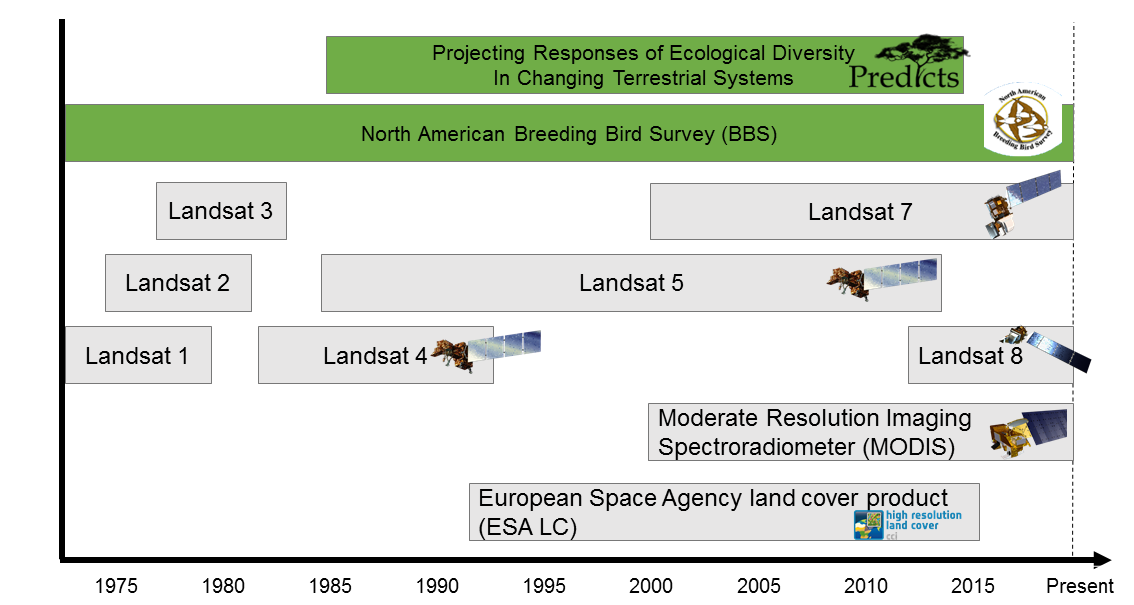
\includegraphics[width=1\textwidth]{chapter2/F01}
\caption{ (\textbf{a}) Locations of 198 species assemblage studies (centroid of each study) coloured by taxonomic group. (\textbf{b}) Diagram of the modelling approach to investigate influences of current and past dissimilarity in photosynthetic activity on species assemblages. The Bray-Curtis index (BC\textunderscript{EVI}) was calculated between pairs (blue arrows) of remote-sensing time series (black solid lines) and of species assemblages (BC\textunderscript{Biodiversity}) collected at paired sites. Independent statistical models were constructed for both current (i - black) and past BC\textunderscript{EVI} of varying length (ii - orange) and their model effects compared (iii – Estimated fixed effects).}
\label{F02_01}
\end{figure}
% -------------------------------------------- %

\subsection{Species trait compilation}
\label{C02_0203}
A species’ size and trophic level are two of the most basic traits for understanding differences in species assemblage structure \citep{Speakman2005,Terborgh2015}. We classified studies into size and trophic bins based on a simple majority: small (>0-9 g animal body mass or > 0-9 cm plant height), medium (10 – 99 g or 10-99 cm) or large species ($\geq$ 100 g or $\geq$ 100 cm), or predominantly herbivore, omnivore, carnivore or detritivore species, by estimating the dominant number of species (simple sum of measurement) within a study. Studies with species of predominantly unknown size or trophic level were removed from the analysis. We thus classified entire studies to the dominant bins as each study’s methodology would likely constrain the average size of animals or plants that can be observed. Data on average adult body mass (in g) were collected for mammals \citep{Jones2009} and birds \citep{Myhrvold2015}, while for plants we used height (in cm) data from the TRY database \citep{Kattge2011}. The estimates of species trophic levels originate from \cite{Kissling2014}, \cite{Wilman2014} and other sources of the literature for invertebrates (obtained from Laura Bentley, Imperial College London, UK). For species for which size or trophic level data were unavailable, we used the genus-wide average for size and the most common trophic level (at least 95\% of all species with data within a genus). We excluded studies (N=8) from further analyses where no clear majority of species (> 50\%) could be assigned to one of the bins (Appendix Figure \ref{SI02_04}), leaving a total of 65 studies with size information and 130 studies with trophic information. 

\subsection{Analysis - Pairwise dissimilarity}
\label{C02_0204}
We linked dissimilarity in photosynthetic activity of vegetation with compositional dissimilarity in species assemblages globally. Specifically, we examined the differential influence of “current” (yr\textunderscript{0}, as the 365 days prior to species assemblage sampling) and “past” (yr\textunderscript{i}, the $i$ years prior to the current year, where $i = 1,..,5$) dissimilarity in photosynthetic activity between spatial pairs of sites (Figure \ref{F02_01}\textbf{b}, Appendix Figure \ref{SI02_03}). We separately considered past periods of increasing lengths (in years, so yr\textunderscript{1}, yr\textunderscript{1:2}, yr\textunderscript{1:3}, yr\textunderscript{1:4}, yr\textunderscript{1:5}). For example, if species assemblage sampling was conducted from the 1\textsuperscript{st} of April until the 15\textsuperscript{th} of July 2008, yr\textunderscript{0} was the 365 days prior to 1\textsuperscript{st} of April 2008, \ie 1\textsuperscript{st} April 2007 – 31\textsuperscript{th} March 2008, and past $i$ years as the period (number of full years $i$) before April 1\textsuperscript{st} 2007.

We used the pairwise Bray-Curtis (BC) index, frequently used in community ecology studies, as a metric to quantify dissimilarity in species assemblage composition between sites \citep{Bray1957,Faith1987,Su2004}. We also considered the binary version of the BC index, the S\o rensen similarity index, to assess whether our results are robust to metric choice. The BC index is a modified Manhattan distance, where the summed distances between values are standardised by the summed values of each site, thus quantifying pairwise dissimilarity from 0 (completely similar) to 1 (entirely different). We used the BC index to measure compositional dissimilarity in local species assemblages (BC\textunderscript{Biodiversity}) between sites within a PREDICTS study. We also applied the BC index to the EVI time series (BC\textunderscript{EVI}) to characterize the dissimilarity between sites in (inter- and intra-annual) vegetation dynamics measured through a proxy representing photosynthetic activity of vegetation in current (yr\textunderscript{0}) and past years (yr\textunderscript{i},where $i = 1,..,5$), which to our knowledge is the first time the BC index has been applied to assess dissimilarity between remotely-sensed time series.

The BC index is calculated between two pairs of sites with PREDICTS species assemblage records or two EVI time-series from sites $x$ and $y$ as follows: 
\begin{equation*}
    BC_{xy} = \frac{( \sum_{k=1}^{n} |x_k - y_k  | )}{ (\sum_{k=1}^{n} x_k + \sum_{k=1}^{n} y_k )}
\end{equation*}
For species assemblages, $x$ and $y$ are the abundances of observed species (n = total number of species) at both sites (non-occurring species were assumed to be absent and set to zero), while for the EVI time series $x$ and $y$ are observed EVI values on the same date (n = total number of dates) in the time series at both sites. The BC\textunderscript{EVI} was calculated on either single or multiple years (yr\textunderscript{i},where $i = 1,..,5$) of EVI time series (Figure \ref{F02_01}\textbf{b}, Appendix Figure \ref{SI02_03}).

Compared to other metrics quantifying dissimilarity between time-series based on remotely-sensed data \citep{Lhermitte2011} the BC\textunderscript{EVI} index has the advantages of (\textbf{a}) taking the actual spectral values as well as distance between them into account, meaning it can be compared between different land-cover types, and (\textbf{b}) using the same method for assessing dissimilarity between species assemblages and between remote-sensing observations. In remote-sensing terms, for any vegetation index (such as EVI), the BC\textunderscript{EVI} index can be interpreted as a measure of absolute differences between two sites in the amount and timing of photosynthetic activity scaled by the total amount of photosynthetic activity available. By calculating the BC\textunderscript{EVI} index on temporal profiles of EVI measurements, we incorporate all differences in EVI between two sites into a single dissimilarity metric. No further scaling has been done as range and unit of the BC\textunderscript{EVI} index values were identical for current and past BC\textunderscript{EVI}.

\subsection{Analysis - Statistical modelling}
\label{C02_0205}
The aim of the statistical modelling is to estimate the influence of current and past BC\textunderscript{EVI} on the BC\textunderscript{Biodiversity} (Figure \ref{F02_01}\textbf{b}). For different time periods (0-5 years) we estimated this influence using separate models rather than an interaction term as current and past BC\textunderscript{EVI} were highly collinear (Random permutation pick: Pearson’s r > 0.9, df = 4046, p < 0.001). A hierarchical modelling approach using generalized linear mixed models (GLMMs) with Gaussian link function was used to fit models of current and past BC\textunderscript{EVI} independently for each time period, taxonomic group, size and trophic bins. GLMMs account for differing sampling methodologies among the PREDICTS studies, by including the “study” as a random intercept in all models. We also allowed the effect of current and past BC\textunderscript{EVI} to vary for each study by incorporating it as a random slope. From each model, we obtained the fixed effects (estimated slope) of the predicted BC\textunderscript{Biodiversity} per unit of current and past BC\textunderscript{EVI}.

As we are primarily interested in the influence of past BC\textunderscript{EVI} (of different periods) on differences in BC\textunderscript{Biodiversity}, we incorporated the influence of current BC\textunderscript{EVI} by transforming the average past BC\textunderscript{EVI} effects (across all permutations) relative to current effects $\frac{Past}{(Current - 1)}$. The resulting ratio describes whether the explicit influence of past BC\textunderscript{EVI} on BC\textunderscript{Biodiversity} is larger (> 0) or smaller (< 0) than the influence of current BC\textunderscript{EVI} (Figure \ref{F02_02}). The precision estimates (predicted standard errors) of the effect of past BC\textunderscript{EVI} were also transformed relative to the precision estimates of current BC\textunderscript{EVI} $\frac{(Imprecision_{past})}{(Imprecision_{current})}$. This helps to visually assess the added imprecision after accounting for the imprecision already present in current BC\textunderscript{EVI}. 

% ---------------- Figure 2 --------------------- %
\begin{figure}[ht]
\centering
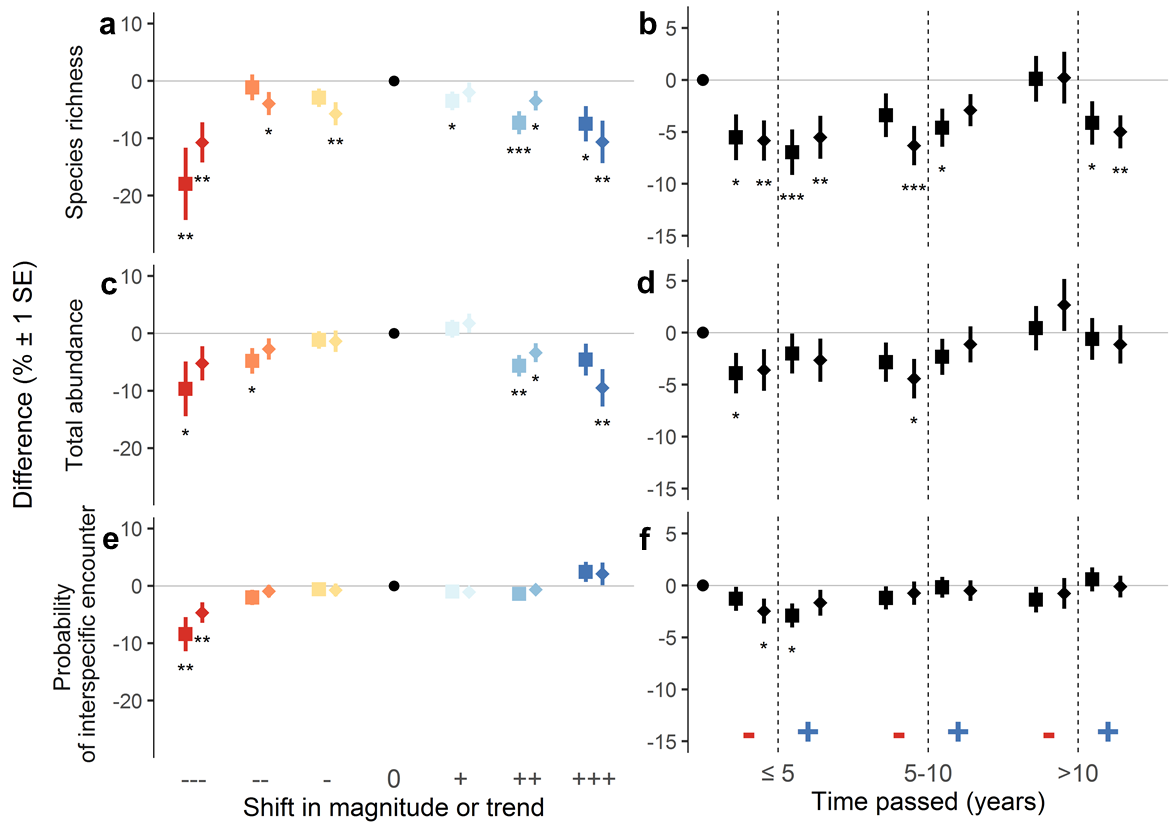
\includegraphics[width=1\textwidth]{chapter2/F02}
\caption{Shows the estimated influence of current (black) and past (orange; assessed over the past five years) BC\textunderscript{EVI} on differences in species assemblages (N = 198 studies). Rugs show the distribution of values from a single randomly selected permutation. The difference between the slopes (arrow) is the relative influence (as ratio) shown in Figures \ref{F02_03} - \ref{F02_06}. Shading shows the predicted standard error.}
\label{F02_02}
\end{figure}
% -------------------------------------------- %

Estimating pairwise comparisons in any regression model would imply substantial pseudo-replication. To account for this, we took the subdiagonal of 100 permuted site-by-site matrices (Appendix Figure \ref{SI02_03}) to construct the GLMMs of 100 separate permutations. This ensures that for each fitted GLMM, our pairwise comparisons are mutually independent subsets \citep{Longacre2005,Newbold2016b}. Fixed effects and standard errors for both current and past BC\textunderscript{EVI} were averaged across all permutations. Furthermore, for each model we calculated a marginal and conditional pseudo R\textsuperscript{2} \citep{Nakagawa2013} and significance estimate \cite{Halekoh2014}, and averaged them across all permutations. As for the fixed effects and precision estimates, the differences in explained marginal variance of past BC\textunderscript{EVI} were assessed relative to the explained marginal variance of current BC\textunderscript{EVI}.

All analyses were performed in R \citep[ver 3.2.2]{RTeam2014} using lme4 \citep[ver. 1.10]{Bolker2009,lme4} for modelling, and vegan \citep[ver. 2.2.3]{Oksanen2015} for the BC calculation of species assemblages data. The processed MODIS data and R-code for the analyses are available on GitHub (\href{https://github.com/Martin-Jung/PastLandSurfaceConditions}{https://github.com/Martin-Jung/PastLandSurfaceConditions}). 

\section{Results}
\label{C02_03}
The compositional dissimilarity of species assemblages (BC\textunderscript{Biodiversity}) increased with between-site dissimilarity in current and past photosynthetic activity (BC\textunderscript{EVI}; current: $\beta$ = 0.289, $\beta_{SE}$ = 0.063, p < 0.001; past yr\textunderscript{1:5}: $\beta$ = 0.334, $\beta_{SE}$ = 0.07, p < 0.001; Figure \ref{F02_02}, Appendix Figure \ref{SI02_05}). When the influence of past BC\textunderscript{EVI} was assessed relative to current BC\textunderscript{EVI}, the BC\textunderscript{Biodiversity} between sites was more pronounced \textendash\ although the imprecision also increased \textendash\ when longer time periods (of up to five years) of past BC\textunderscript{EVI} were considered (Figure \ref{F02_03}). Furthermore, the consideration of past BC\textunderscript{EVI} calculated up to five years prior to current BC\textunderscript{EVI} increased the relative explained marginal variance by 16.7\% (Appendix Table \ref{SIT02_01}). We ensured that the BC index was robust with regards to varying time period lengths (Appendix Figure \ref{SI02_06}), spatial autocorrelation (Appendix Figure \ref{SI02_07}) and other temporal and geographic biases (Appendix Figure \ref{SI02_08}). Similar results were found by using a different metric of species assemblage composition, the S\o rensen similarity index, that does not require species abundance estimates (Appendix Figure \ref{SI02_09}).

% ---------------- Figure 3 --------------------- %
\begin{figure}[ht]
\centering
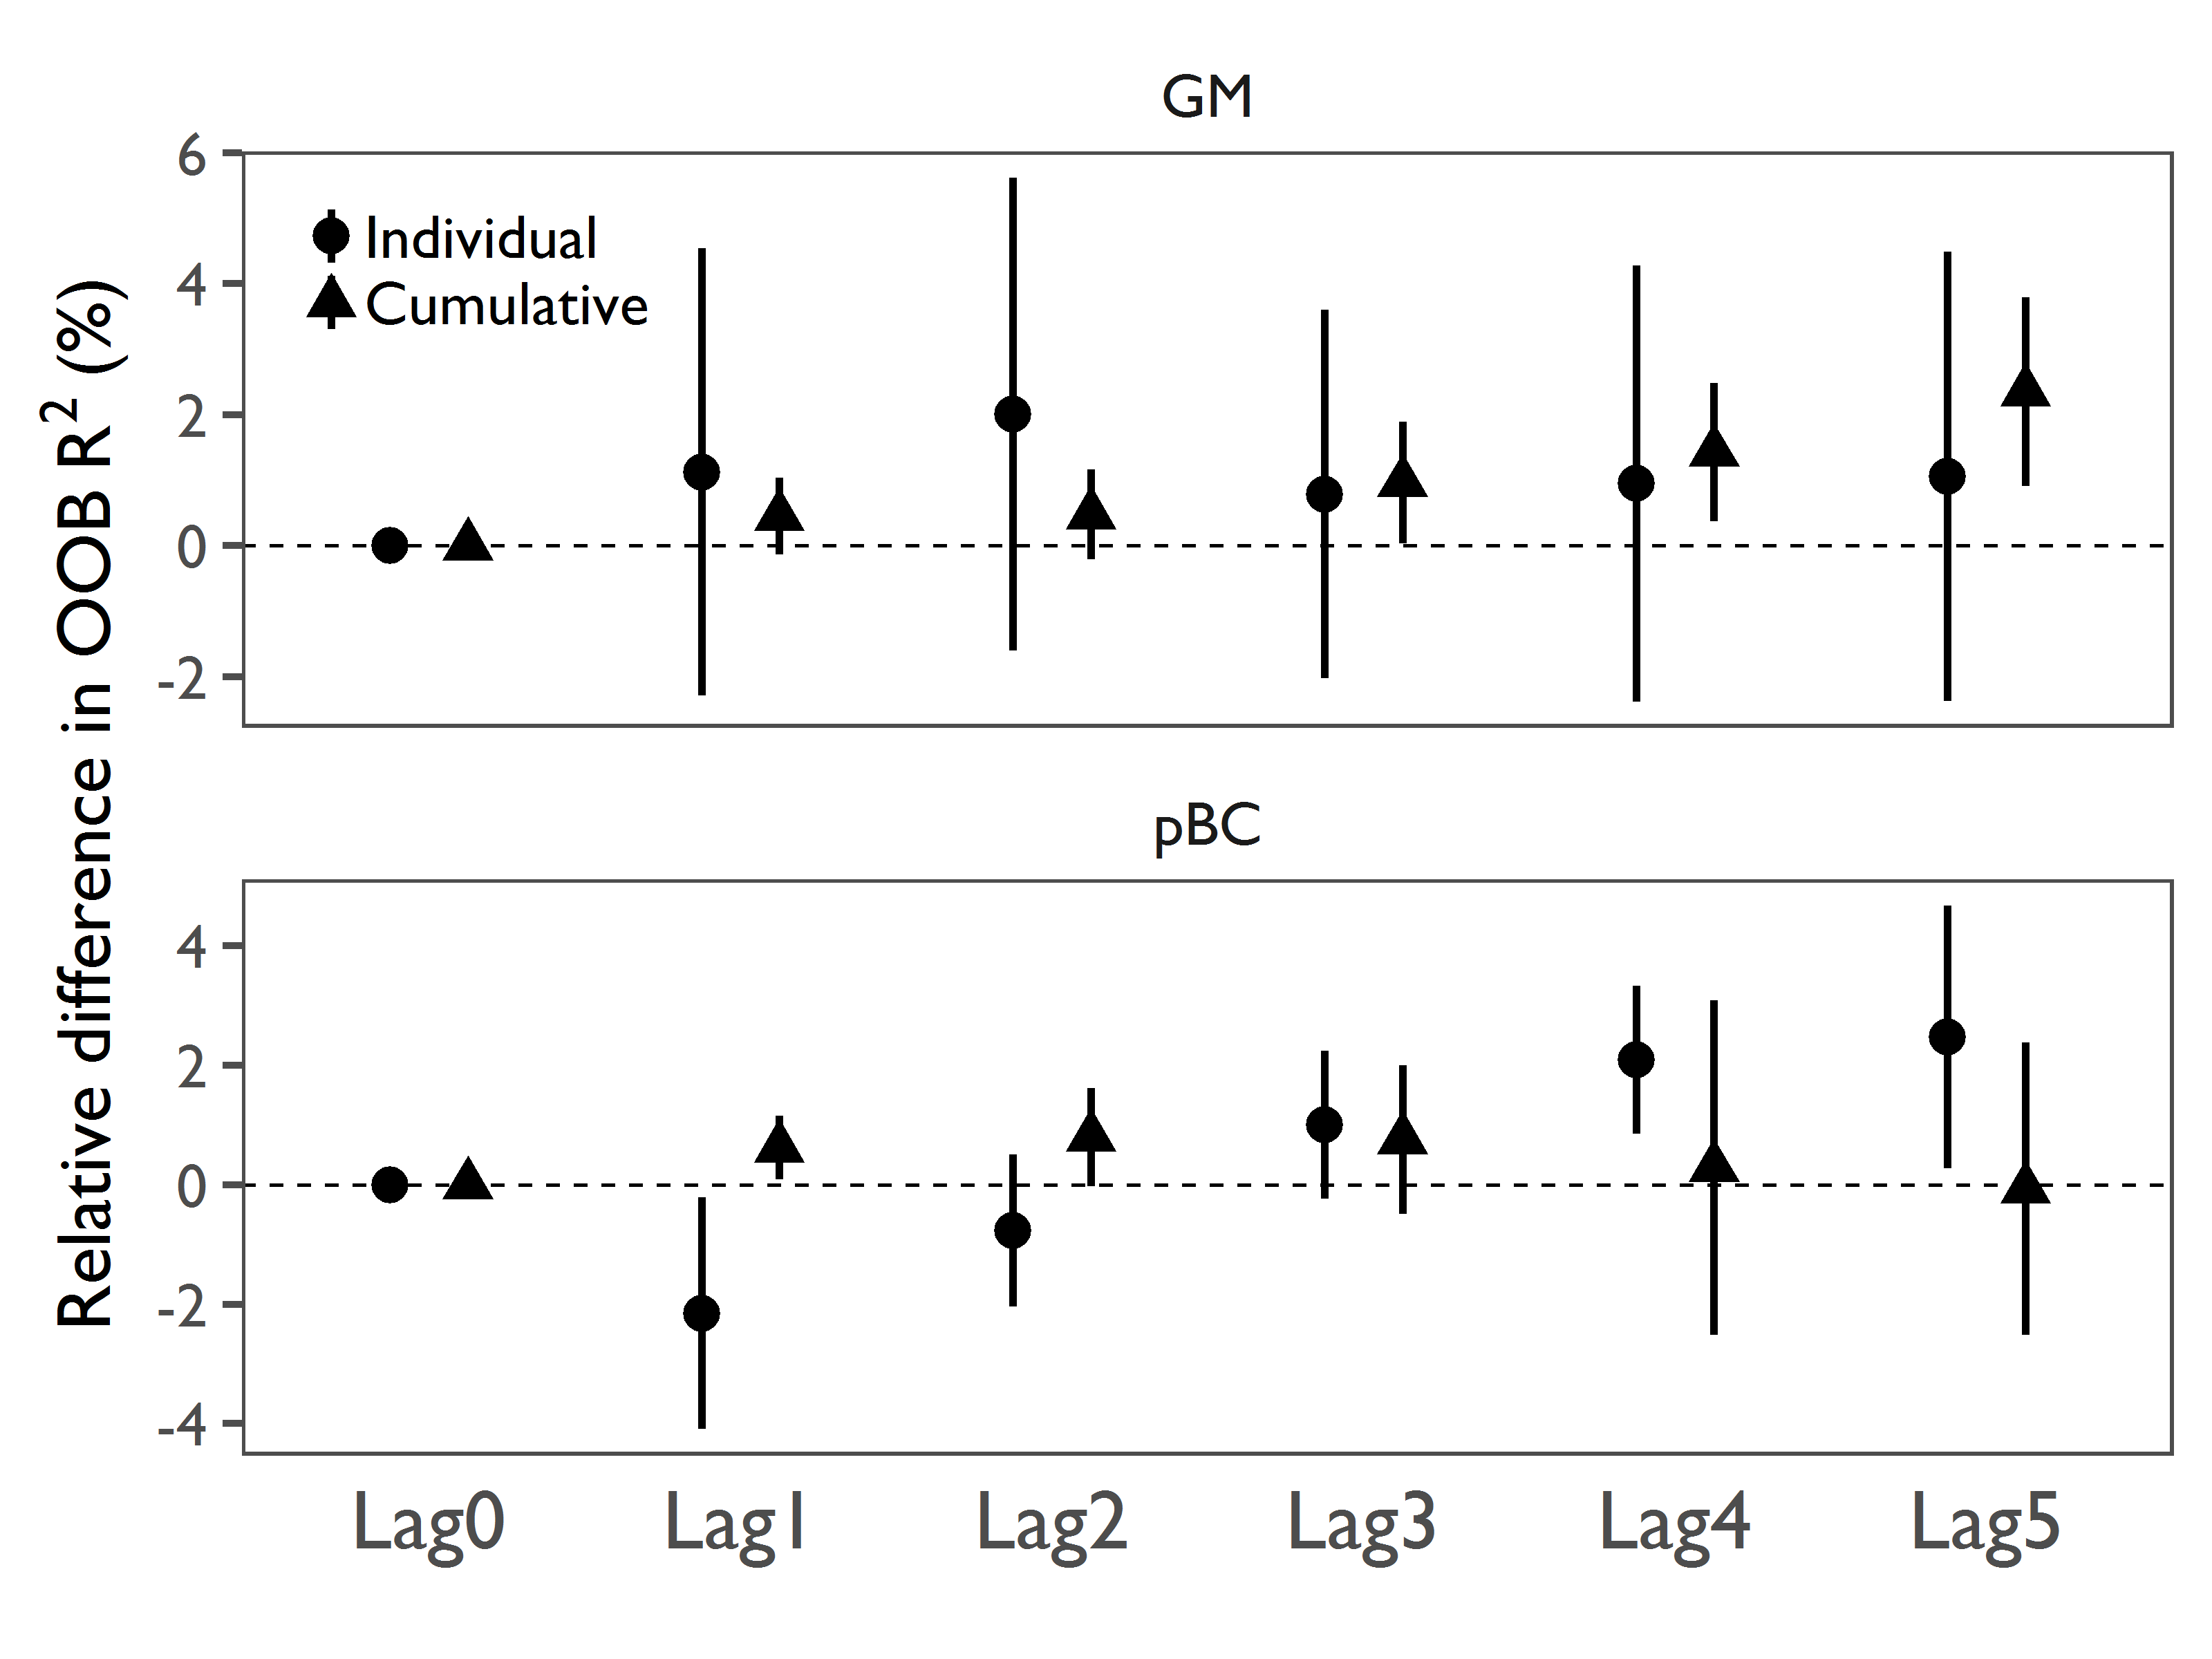
\includegraphics[width=1\textwidth]{chapter2/F03}
\caption{Overall influence on species assemblage composition of past BC\textunderscript{EVI} relative to current BC\textunderscript{EVI}, estimated individually for past periods of differing length (yr\textunderscript{1} to yr\textunderscript{1:5}, representing 1 year and up to 5 years current BC\textunderscript{EVI}). The predicted effects and their precision (standard error) of past BC\textunderscript{EVI} (yr\textunderscript{1:5}) on dissimilarity in species assemblages were transformed relative to the effects and precision of current BC\textunderscript{EVI} (yr\textunderscript{0}). Note that error bars indicate the predicted precision of differences in past BC\textunderscript{EVI} relative to the precision of differences in current BC\textunderscript{EVI}. Positive values indicate that differences in past BC\textunderscript{EVI} lead to greater differences in species assemblages than differences in current BC\textunderscript{EVI}.}
\label{F02_03}
\end{figure}
% -------------------------------------------- %
The influence of past BC\textunderscript{EVI} on species assemblages was found to vary among taxonomic groups and time periods considered (Figure \ref{F02_04}). Dissimilarity in plant, invertebrate, reptilian and bird assemblage composition increased with increasing BC\textunderscript{EVI} of the past two to five years. In contrast, the influence of past BC\textunderscript{EVI} on mammalian assemblages was greatest for the first two years relative to the influence of current BC\textunderscript{EVI} but decreased when longer periods of three to five years of past BC\textunderscript{EVI} were considered. Meanwhile, amphibian assemblages were more influenced by current than past BC\textunderscript{EVI} between sites (Figure \ref{F02_04}).
% ---------------- Figure 4 --------------------- %
\begin{figure}[ht]
\centering
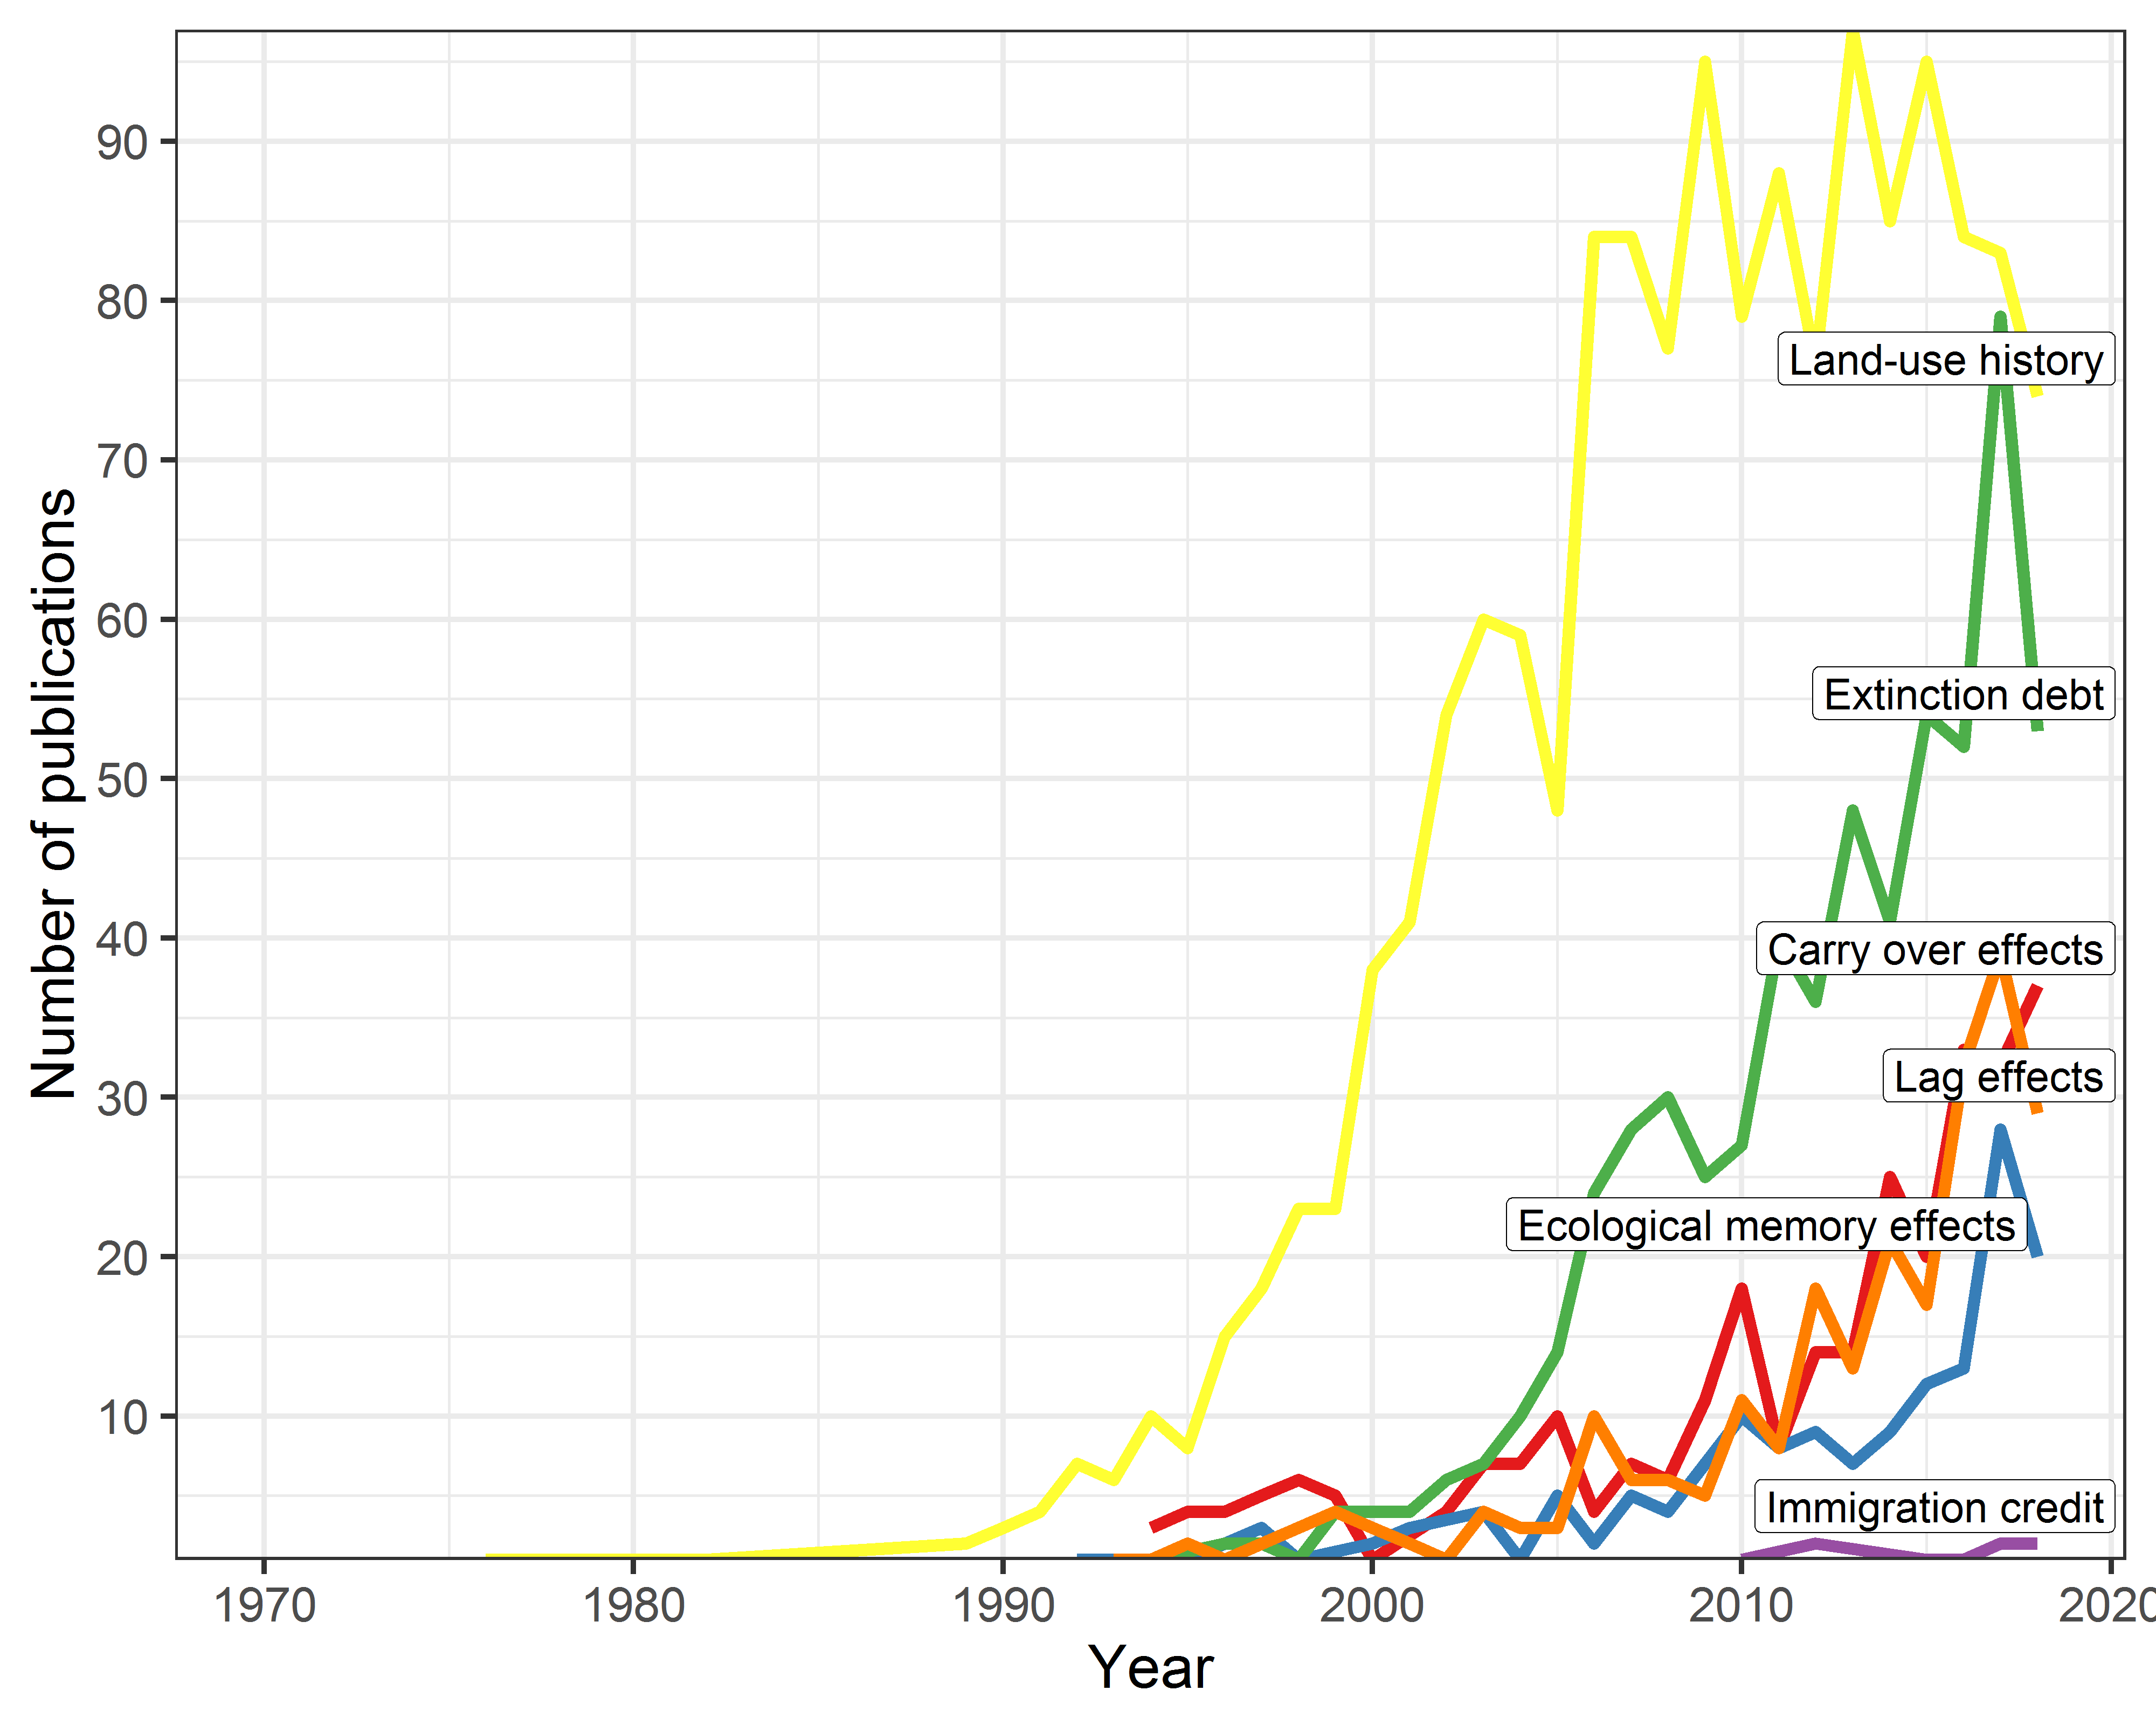
\includegraphics[width=1\textwidth]{chapter2/F04}
\caption{Influence of past BC\textunderscript{EVI} on species assemblage composition across different taxonomic groups. Visualized as relative influence of past BC\textunderscript{EVI} compared to current BC\textunderscript{EVI} as described in Figure \ref{F02_03}. The number of studies and contributing sites (N | N\textunderscript{Sites}) is indicated for each group.}
\label{F02_04}
\end{figure}
% -------------------------------------------- %
The influence of past BC\textunderscript{EVI} differed with respect to body size (Figure \ref{F02_05}). Species assemblages that were dominated by small- (> 0-9 g body mass) and medium-sized (10-99 g) mammals were more influenced by differences in BC\textunderscript{EVI} over the past one to three years, while the influence on assemblages dominated by larger ($\geq$ 100 g) mammals increased with longer time periods. Compared to assemblages dominated by medium-sized birds, assemblages of large bird species were up to five times more influenced by past relative to current BC\textunderscript{EVI}. For plant assemblages with available information on size, we found that assemblages dominated by medium-sized plants were more influenced by past BC\textunderscript{EVI} compared to those assemblages dominated by larger plant species (Figure \ref{F02_05}). 
% ---------------- Figure 5 --------------------- %
\begin{figure}[ht]
\centering
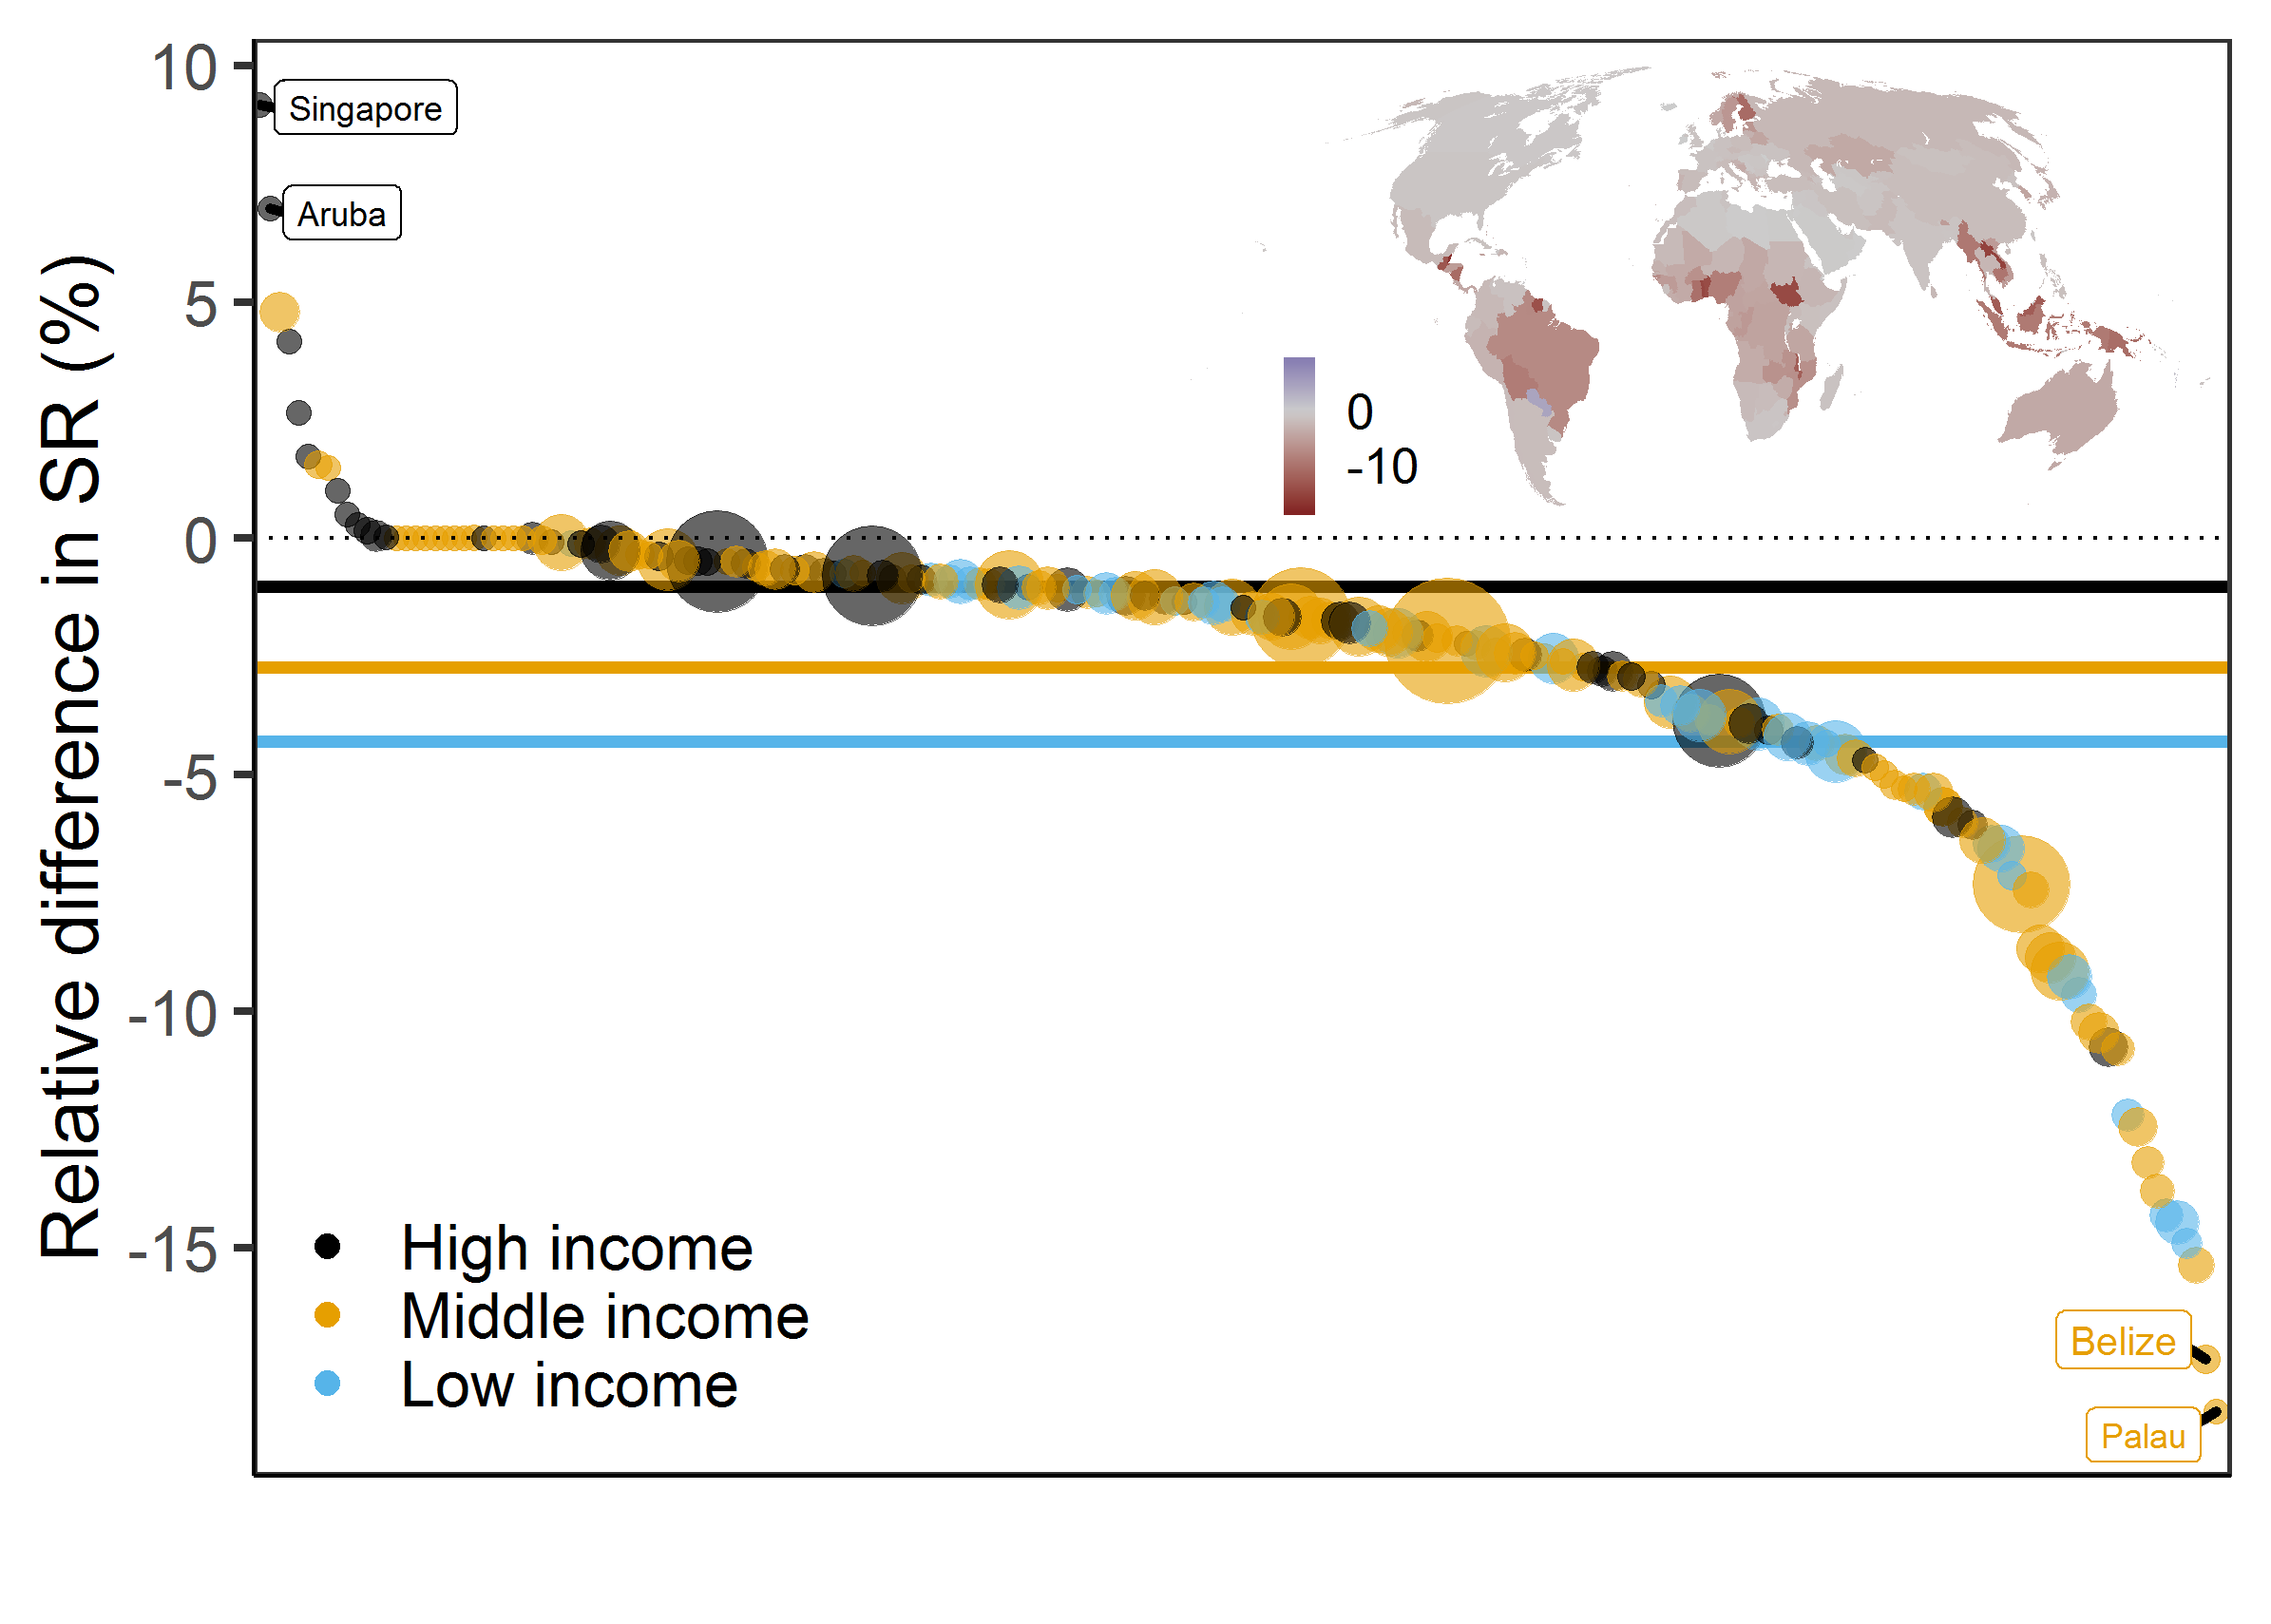
\includegraphics[width=1\textwidth]{chapter2/F05}
\caption{Influence of past BC\textunderscript{EVI} on species assemblages (N = 65) of predominantly small (> 0 - 9), medium (10 - 99) and large sized animals and plants ($\geq$ 100). Available size was measured as adult body mass (in g) for all birds (blue) and mammals (red) and height for plants (green, in cm). Within each study all species were binned into one size group and the study categorized based on which size group is predominant across all sites. The bar chart shows the number of studies that contributed to each taxonomic group and body size bin. Visualized as relative influence of past BC\textunderscript{EVI} compared to current BC\textunderscript{EVI} as described in Figure \ref{F02_03} and methods.}
\label{F02_05}
\end{figure}
% -------------------------------------------- %
Differences among trophic levels were also seen in the influence of past BC\textunderscript{EVI} on BC\textunderscript{Biodiversity} and increased with longer time periods considered (Figure \ref{F02_06}). Species assemblages dominated by omnivorous and herbivorous assemblages were more influenced by past BC\textunderscript{EVI} of even one year relative to the influence of current BC\textunderscript{EVI}, while detritivores assemblages were only more influenced by past BC\textunderscript{EVI} if periods of the past three years were considered (Figure \ref{F02_06}). In contrast, studies with predominantly carnivorous species were more influenced by current BC\textunderscript{EVI} and showed no overall trend with longer time periods of past BC\textunderscript{EVI} considered (Figure \ref{F02_06}). 
% ---------------- Figure 6 --------------------- %
\begin{figure}[hb]
\centering
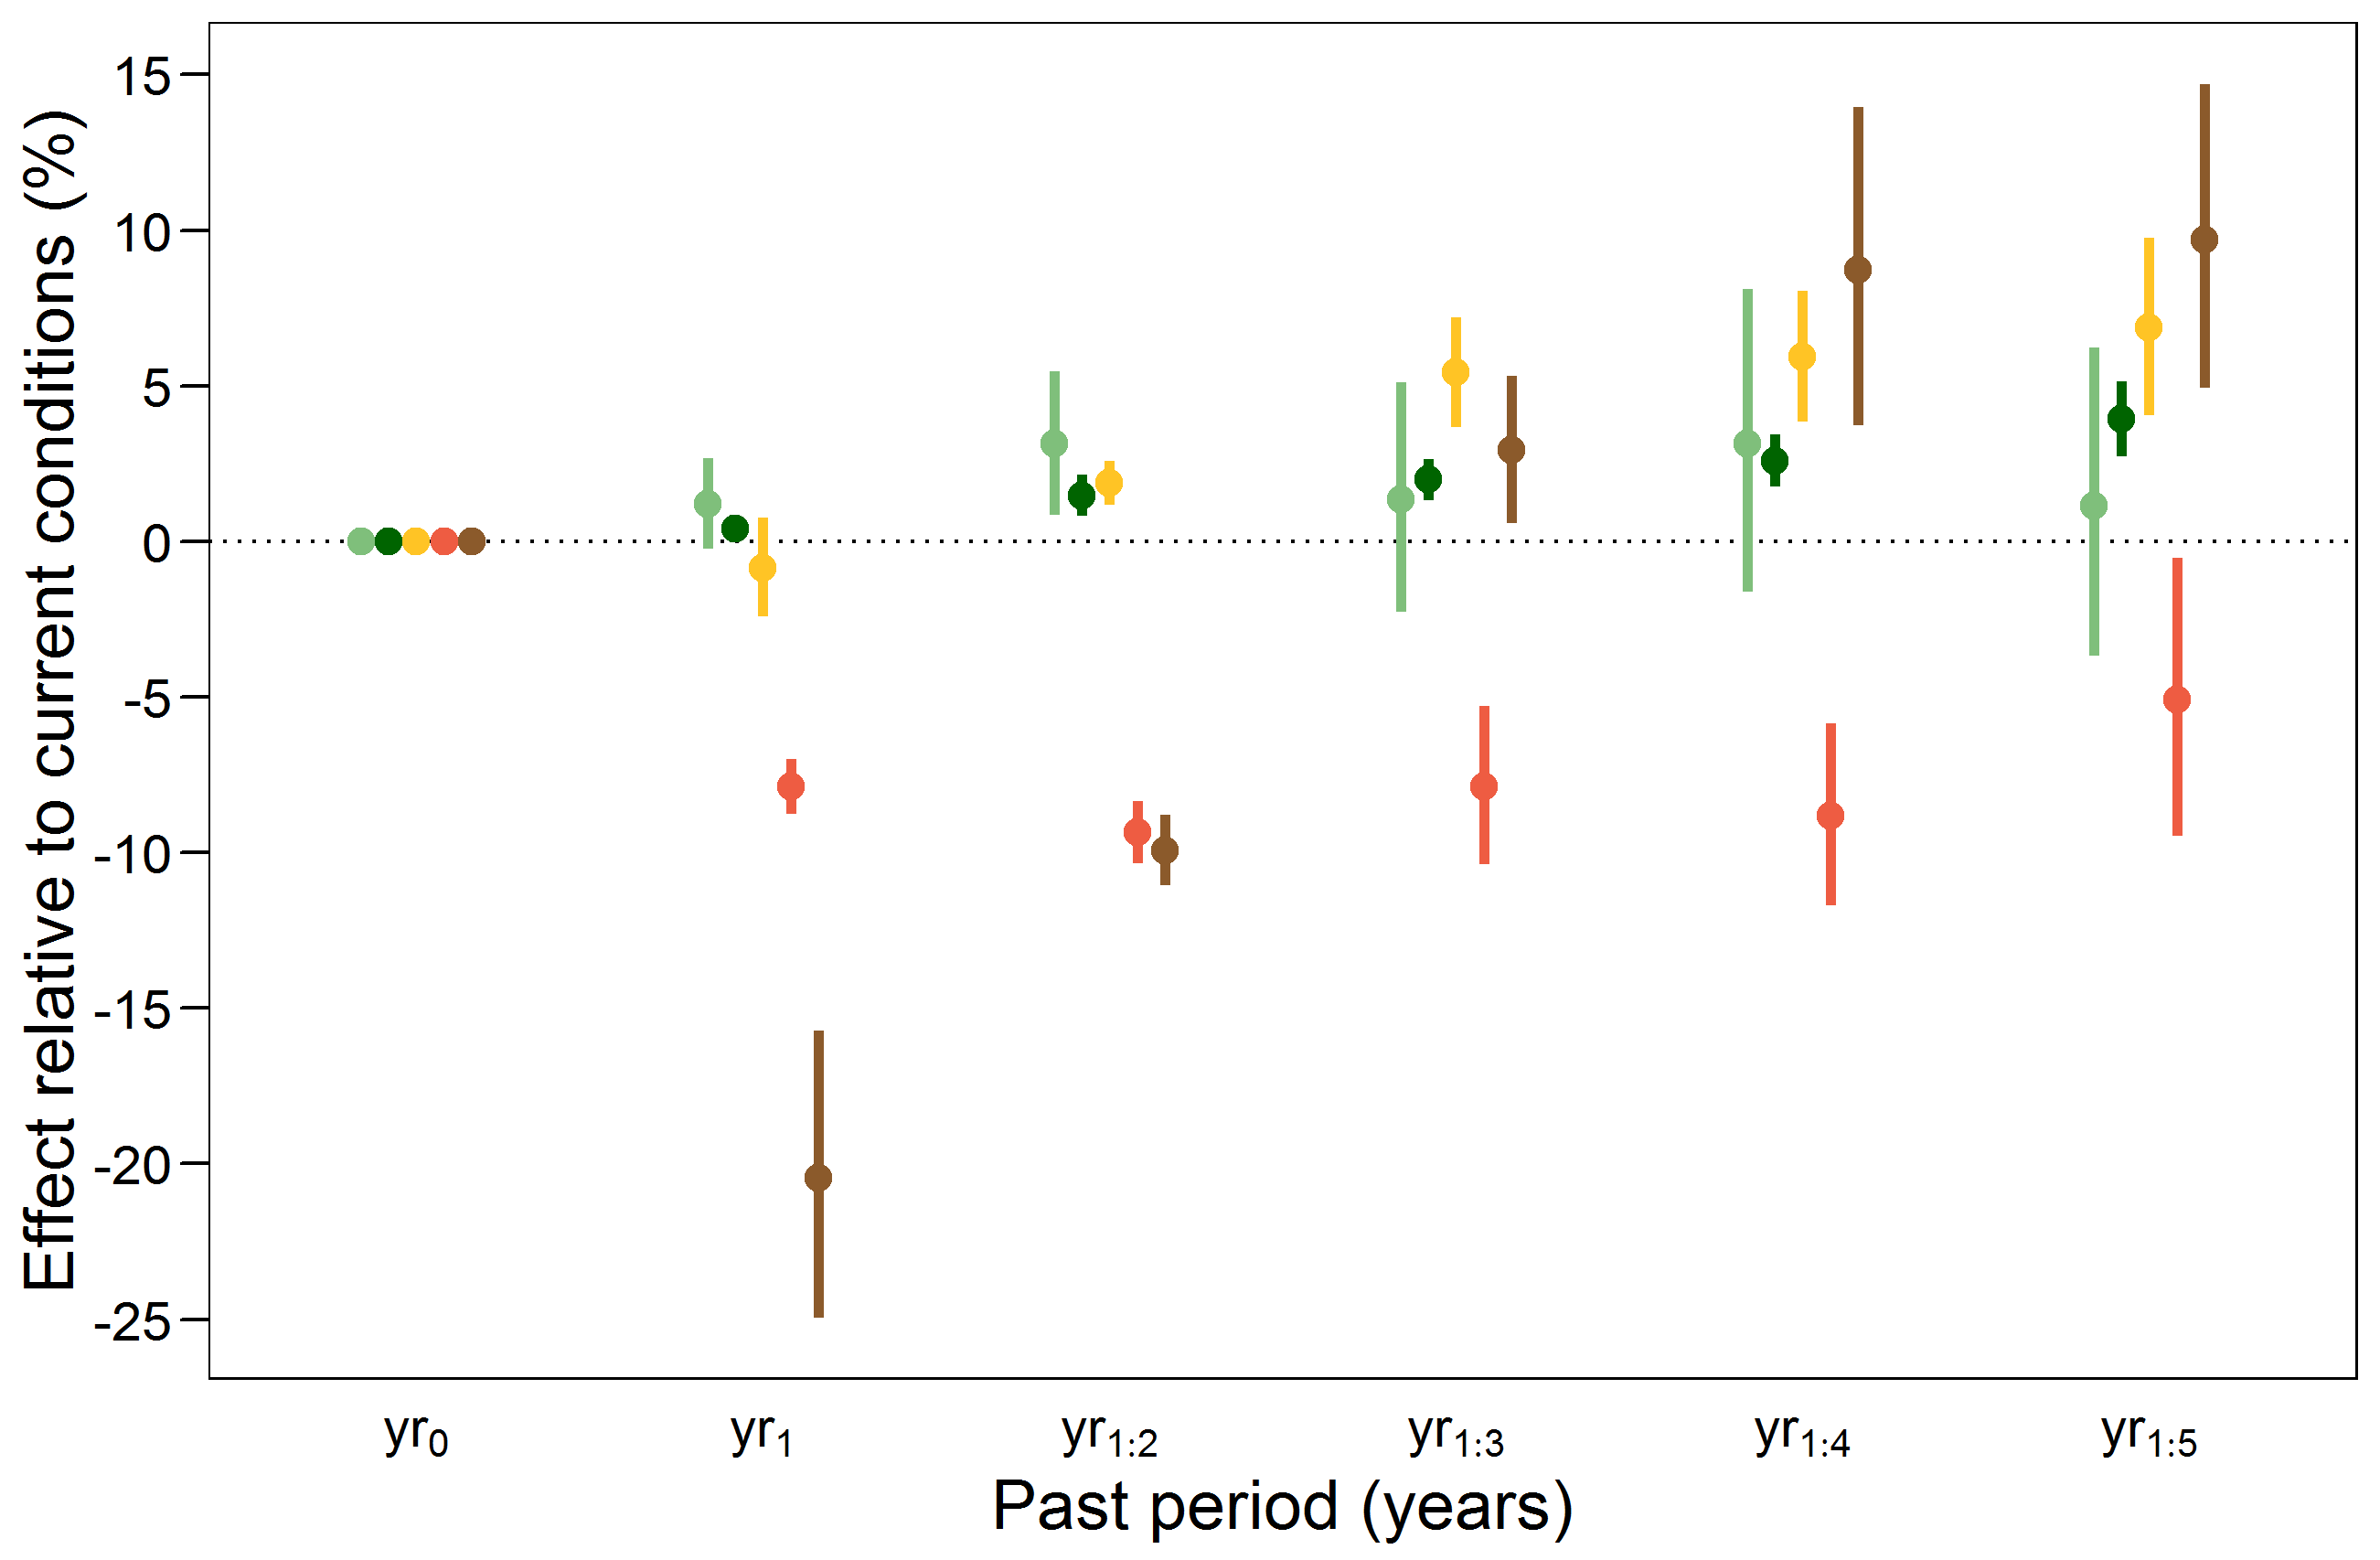
\includegraphics[width=1\textwidth]{chapter2/F06}
\caption{Influence of past BC\textunderscript{EVI} on trophic bins across studies (N = 130). Within each study all species were categorized as one trophic level and the study categorized based on which level is predominant across all sites. Colours indicate the influence of current and past BC\textunderscript{EVI} for autotroph plants (light green, N=28), herbivores (dark green, N=49), omnivores (yellow, N= 29), carnivores (red, N=13) and detritivores (brown, N=9). Visualized as relative influence of past BC\textunderscript{EVI} compared to current BC\textunderscript{EVI} as described in Figure \ref{F02_03}.}
\label{F02_06}
\end{figure}
% -------------------------------------------- %

\section{Discussion}
\label{C02_04}
The main aim of this study was to investigate if between-site dissimilarity in current and past photosynthetic activity of vegetation (BC\textunderscript{EVI}) can predict compositional dissimilarity in sites’ species assemblages (BC\textunderscript{Biodiversity}). In contrast to previous PREDICTS-based studies that used discrete measures of current land use and land-use intensity \citep{Newbold2015,Newbold2016b}, we used a continuous measure of between-site dissimilarity in remotely-sensed photosynthetic activity that summarises (inter- and intra-annual) vegetation dynamics in a single metric (the BC\textunderscript{EVI}). We explicitly differentiated between current (the full year prior to species assemblage sampling) and past BC\textunderscript{EVI} (periods of up to five years before current) that could have influenced compositional dissimilarity in species assemblages. Similar to previous studies using the same dataset to analyse compositional differences with respect to land use \citep{Newbold2016b}, we found that sites with more different current BC\textunderscript{EVI} also had more different species assemblages (Figure \ref{F02_02}, Appendix Figure \ref{F02_05}). However, the BC\textunderscript{EVI} calculated over five years prior to biodiversity sampling had, on average, an even greater influence on between-site dissimilarity in species assemblage composition compared to current BC\textunderscript{EVI} (Figure \ref{F02_03}). This pattern was consistent across most taxonomic (Figure \ref{F02_04}) and functional groups (Figure \ref{F02_05} and \ref{F02_06}). Here we discuss potential causes and implications of the observed patterns as well as factors that can affect the BC\textunderscript{EVI}.

\subsection{Potential drivers of dissimilarities in photosynthetic activity}
\label{C02_0401}
Dissimilarities in photosynthetic activity can be caused by many natural \citep{Fensholt2012,Zhu2016} and/or anthropogenic factors \citep{Lambin2006,Turner2007}. The latter were likely the dominant cause of current differences between sites in our analyses, given that the PREDICTS database includes only studies of mostly small geographic extent with a difference in current human land use or land-use intensity \citep{Hudson2016}, however climatic factors likely influence the BC\textunderscript{EVI} as well. Dissimilarity metrics of photosynthetic activity can be considered a coarse approximation of overall differences in land use and land cover as well as in climatic and other abiotic factors between sites \citep{Linderman2005,Lupo2007,Lhermitte2011}. Past studies have linked differences in vegetation dynamics with the use intensity of agriculture \citep{Estel2015,Tong2017}, land-cover change such as deforestation events \citep{Lambin1994,DeVries2015b}, or land degradation and intensification \citep{dejong2011, Mueller2014}. The BC\textunderscript{EVI}, similar to other metrics used to monitor remotely-sensed vegetation dynamics \citep{Linderman2005,Rowhani2008,Lhermitte2011}, quantifies dissimilarity in photosynthetic activity across different types of land cover, by exploiting both distance between time series (the absolute difference in EVI data) and amount (area under the time series) of photosynthetic activity. Besides differences in land use and land cover, dissimilarity metrics such as the BC\textunderscript{EVI} will also be affected by climatic differences in precipitation and radiation \citep{Fensholt2012,Zhu2016}, soil properties \citep{Ahmed2017} or plant species composition \citep{He2009}. The BC\textunderscript{EVI} thus quantifies dissimilarity in vegetation dynamics caused by both natural and anthropogenic factors affecting EVI time-series.

However, some natural and anthropogenic factors cannot be directly quantified from remotely-sensed time series \citep{Peres2006,Turner2007} and the BC\textunderscript{EVI} is limited to those aspects that affect photosynthetic activity of vegetation. Furthermore, because of the way the BC\textunderscript{EVI} is calculated, it can only represent overall dissimilarity in photosynthetic activity but cannot be used to infer directionality or timing of change (vegetation regrowth or loss, disturbances such as fires, etc.). By using entire periods (\ie five full years, instead of the fifth year) it is not possible to disentangle overall dissimilarity and any ‘change’ in photosynthetic activity \textit{per se} \citep[cf.][]{Linderman2005}. Calculating the BC\textunderscript{EVI} index on longer time periods did not affect the possible range of observed values (Appendix Figure \ref{SI02_06}), however it likely enhances our ability to capture aspects of past variability in vegetation dynamics caused by either natural and/or anthropogenic drivers. We recommend that future studies evaluate the performance of the BC\textunderscript{EVI} relative to other time-series dissimilarity metrics. 

\subsection{Influences of current and past dissimilarities in photosynthetic activity on biodiversity}
\label{C02_0402}
Our results suggest that species assemblage composition was consistently more dissimilar between sites with greater current dissimilarity in photosynthetic activity of vegetation (as quantified by the BC\textunderscript{EVI}) (Figure \ref{F02_02}, Appendix Figure \ref{F02_05}). This is in line with previous studies that have correlated some measurement of dissimilarity in current ‘environmental heterogeneity’ with compositional dissimilarity in species assemblage composition \citep{Buckley2008,He2009,Newbold2016b}. However species assemblages might also be explicitly influenced by past dissimilarity in photosynthetic activity \citep{Johnson2008,Watson2014,Ogle2015,Perring2015}. 

Differences in past BC\textunderscript{EVI} were on average more correlated with dissimilarity in species assemblages than differences in current BC\textunderscript{EVI} (Figure \ref{F02_02}-\ref{F02_03}). This could indicate that past dissimilarity in photosynthetic activity continues to have a lasting influence or memory effect on species assemblages \citep{Ogle2015}, especially as the effect generally increased as longer periods of past BC\textunderscript{EVI} were considered (Figure \ref{F02_03}), therefore increasing the likelihood that past changes in photosynthetic activity of vegetation have been captured. Longer periods of past BC\textunderscript{EVI} also increased the explained marginal variance (Appendix Table \ref{SIT02_01}), although most of the variance was already explained by differences in study identity (thus by sampling methods and local factors). The marginal variance explained was modest, but comparable to other broad-scale studies using the same species assemblage dataset \citep{Newbold2014b,DePalma2015,Jung2016}. It is a limitation that we used data from a wide variety of sources \citep{Hudson2016}, which were typically not designed to study lag or memory effects of past changes in land-surface conditions such as photosynthetic activity. At many of the sites in our analyses inter-annual photosynthetic activity could have remained relatively stable during the past five years, which would reduce our ability to differentiate any effects of past BC\textunderscript{EVI}. Similarly, any dissimilarity in photosynthetic activity among pairs of sites could have been even greater before the monitoring period of MODIS (since year 2000), which we were unable to quantify using these data. 

Notably, species assemblages of some taxonomic groups were more dissimilar in composition than others if past dissimilarity in photosynthetic activity was considered (Figure \ref{F02_04}). The influence of past BC\textunderscript{EVI} on reptilian species assemblages was large (\textasciitilde35\% more different than current) even for the relatively short period of five years (Figure \ref{F02_04}). Potentially many of the sites of the reptilian studies have been subjected to relatively recent changes in photosynthetic activity of vegetation prior to species assemblage sampling. Indeed, in one of the studies, \cite{Woinarski2009} explicitly suggested an influence of past fires and varying grazing intensity on reptilian species assemblages. In contrast, we found that amphibian species assemblages were less influenced by past compared to current BC\textunderscript{EVI}, despite being more influenced by current BC\textunderscript{EVI} than all other taxonomic groups (Appendix Figure \ref{F02_05}). An explanation could be that most compositional differences between amphibian assemblages that are attributable to past dissimilarities in photosynthetic activity are already explained by current dissimilarity in BC\textunderscript{EVI}. It may be that amphibian assemblages are more influenced by factors other than past photosynthetic activity (such as microclimatic conditions). Disentangling broad taxonomic groups into functional groups may assist in highlighting specific responses to past dissimilarities in photosynthetic activity.

Differences in functional traits can influence species responses to dissimilarity in photosynthetic activity \citep{Newbold2013,DePalma2015} and we expect that on average smaller species would be more affected by recent dissimilarity in photosynthetic activity (a few years before sampling). Our results confirm this assumption as species assemblages with predominantly small- or medium-sized plants, birds and mammals were relatively more influenced by past BC\textunderscript{EVI} over two to three years prior to sampling than by current BC\textunderscript{EVI} (Figure \ref{F02_05}). Smaller species tend to live shorter lives and disperse less far than larger species \citep{Brown2004,Thomson2011,Stevens2014}, which might make them more susceptible to dissimilarity in photosynthetic activity shortly before sampling \citep{Watson2014}. Similar to previous studies \citep{Jakovac2016} we showed that smaller plant species were more influenced by past dissimilarity in photosynthetic activity over up to five years prior to sampling as quantified by the BC\textunderscript{EVI} (Figure \ref{F02_05}). For assemblages dominated by larger plants we did not detect such an influence and it is likely that the considered period (five years) was too short to show measurable influences. Overall our results indicate that assemblages dominated by smaller species might have been more influenced by past dissimilarity in photosynthetic activity,  possibly because of carry-over or ecological memory effects \citep{Harrison2011,Ogle2015}. Other functional traits, such as generation time or dispersal capability \citep{Watson2014}, as well as better coverage of existing traits for underrepresented taxonomic groups could assist in further disentangling these influences especially given the large uncertainty across most influences (Figure \ref{F02_05}). 

The response of species assemblages to dissimilarities in past photosynthetic activity also differed between trophic bins. Except for carnivores, species assemblage composition of all trophic bins were on average more influenced by longer periods of past rather than by current dissimilarity in photosynthetic activity, as measured by BC\textunderscript{EVI} (Figure \ref{F02_06}). Yet we found noticeable lags in the observed influence of past BC\textunderscript{EVI} with varying time periods. Relative to the influence of current BC\textunderscript{EVI}, the influence of past BC\textunderscript{EVI} was larger for assemblages dominated by autotrophs, herbivores, omnivores and detritivores (Figure \ref{F02_06}). Notably, detritivores were more correlated with past BC\textunderscript{EVI} only if past periods of three to four years were considered. This supports previous studies which have shown that plant-dependant species are highly sensitive to variability in current and past photosynthetic activity as quantified by remote sensing \citep{Pettorelli2006,Newton2014}. In contrast, we found predominantly carnivorous assemblages to be less influenced by past BC\textunderscript{EVI} compared to current BC\textunderscript{EVI} regardless of the considered time period. Possibly, carnivore abundance was more influenced by contemporary prey density \citep{Terborgh2015} than past dissimilarity in photosynthetic activity (Figure \ref{F02_06}). Because of a lack of data for carnivores and herbivores co-occurring at the same site, we were unable to investigate such interactions. 

\section{Study implications and conclusions}
\label{C02_05}
Knowledge about past dissimilarities in land-surface conditions, such as photosynthetic activity of vegetation, and their influence on species assemblages is important for both the design of ecological studies and interpretation of dissimilarities in current composition of species assemblages. We found that sites with more dissimilar past than current photosynthetic activity (as quantified by the BC\textunderscript{EVI}) were more strongly correlated with compositional dissimilarity in local species assemblages among spatial pairs of nearby sites. Ignoring such past influences can lead to biased biodiversity estimates by not accounting for extinction debts or immigration credits still to be paid \citep[see ][]{Tilman1994} or lasting ecological memory and carry-over effects because of higher variability in past photosynthetic activity \citep{Rowhani2008,Cole2015,Ogle2015}. We suggest that future broad scale studies investigating biodiversity responses to environmental changes should explicitly consider legacy effects that influence species assemblages in a study area and we demonstrate how remote sensing can help to quantify such effects globally. Our approach could be extended to incorporate differences in the vegetation dynamics of the surrounding landscape. There is some evidence that landscape-wide temporal differences in photosynthetic activity can affect species assemblage composition \citep{Manning2009,Fernandez2016}. In conclusion, we have demonstrated that compositional dissimilarity of species assemblages, of various taxonomic and functional groups, are not only influenced by dissimilarity in current photosynthetic activity, but also by dissimilarity in past photosynthetic activity over the last five years. Future studies should investigate the influence of disturbance events and directionality of changes in photosynthetic activity for more than five years before local biodiversity sampling.

%\section{Acknowledgements}
%\label{C02_06}
%We thank all PREDICTS data contributors for their biodiversity data, which was collated using support from the Natural Environment Research Council (NERC, grant number: NE/J011193/2). PREDICTS is endorsed by the GEO BON. This study has benefited from publicly available data from the TRY initiative on plant traits (\href{http://www.try-db.org}{http://www.try-db.org}). We acknowledge the University of Sussex, School of Life Sciences for a doctoral training grant and for providing computing facilities.

\section{Data availability}
\label{C02_06}
Extracted MODIS data and pairwise biodiversity permutations are available on GitHub. A 2016 snapshot of the PREDICTS database has been openly released earlier\\ (\doi{10.5519/0066354}).

\clearpage
%\bibliography{content/01Chapter}

%\appendix
%\begingroup
%  Blank

%\endgroup
